% Contains subfigures - use inside a figure environment
\begin{subfigure}{\textwidth}
  \centering
  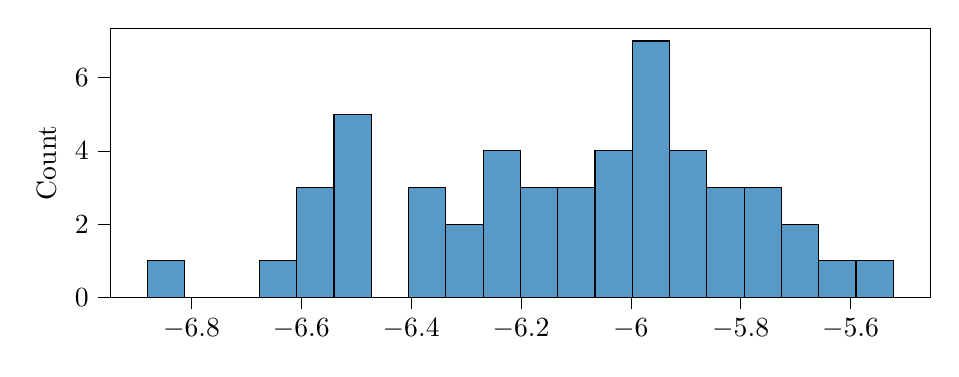
\begin{tikzpicture}
    \definecolor{color0}{rgb}{0.12156862745098,0.466666666666667,0.705882352941177}
    \begin{axis}[
    tick align=outside,
    tick pos=left,
    x grid style={white!69.0196078431373!black},
    xmin=-6.94795252966014, xmax=-5.45416511327468,
    xtick style={color=black},
    y grid style={white!69.0196078431373!black},
    ylabel={Count},
    ymin=0, ymax=7.35,
    ytick style={color=black},
    width=12cm, height=5cm
    ]
    \draw[draw=black,fill=color0,fill opacity=0.75] (axis cs:-6.88005310164262,0) rectangle (axis cs:-6.8121536736251,1);
    \draw[draw=black,fill=color0,fill opacity=0.75] (axis cs:-6.8121536736251,0) rectangle (axis cs:-6.74425424560758,0);
    \draw[draw=black,fill=color0,fill opacity=0.75] (axis cs:-6.74425424560758,0) rectangle (axis cs:-6.67635481759006,0);
    \draw[draw=black,fill=color0,fill opacity=0.75] (axis cs:-6.67635481759006,0) rectangle (axis cs:-6.60845538957254,1);
    \draw[draw=black,fill=color0,fill opacity=0.75] (axis cs:-6.60845538957254,0) rectangle (axis cs:-6.54055596155502,3);
    \draw[draw=black,fill=color0,fill opacity=0.75] (axis cs:-6.54055596155502,0) rectangle (axis cs:-6.4726565335375,5);
    \draw[draw=black,fill=color0,fill opacity=0.75] (axis cs:-6.4726565335375,0) rectangle (axis cs:-6.40475710551998,0);
    \draw[draw=black,fill=color0,fill opacity=0.75] (axis cs:-6.40475710551998,0) rectangle (axis cs:-6.33685767750246,3);
    \draw[draw=black,fill=color0,fill opacity=0.75] (axis cs:-6.33685767750246,0) rectangle (axis cs:-6.26895824948493,2);
    \draw[draw=black,fill=color0,fill opacity=0.75] (axis cs:-6.26895824948493,0) rectangle (axis cs:-6.20105882146741,4);
    \draw[draw=black,fill=color0,fill opacity=0.75] (axis cs:-6.20105882146741,0) rectangle (axis cs:-6.13315939344989,3);
    \draw[draw=black,fill=color0,fill opacity=0.75] (axis cs:-6.13315939344989,0) rectangle (axis cs:-6.06525996543237,3);
    \draw[draw=black,fill=color0,fill opacity=0.75] (axis cs:-6.06525996543237,0) rectangle (axis cs:-5.99736053741485,4);
    \draw[draw=black,fill=color0,fill opacity=0.75] (axis cs:-5.99736053741485,0) rectangle (axis cs:-5.92946110939733,7);
    \draw[draw=black,fill=color0,fill opacity=0.75] (axis cs:-5.92946110939733,0) rectangle (axis cs:-5.86156168137981,4);
    \draw[draw=black,fill=color0,fill opacity=0.75] (axis cs:-5.86156168137981,0) rectangle (axis cs:-5.79366225336229,3);
    \draw[draw=black,fill=color0,fill opacity=0.75] (axis cs:-5.79366225336229,0) rectangle (axis cs:-5.72576282534477,3);
    \draw[draw=black,fill=color0,fill opacity=0.75] (axis cs:-5.72576282534477,0) rectangle (axis cs:-5.65786339732725,2);
    \draw[draw=black,fill=color0,fill opacity=0.75] (axis cs:-5.65786339732725,0) rectangle (axis cs:-5.58996396930973,1);
    \draw[draw=black,fill=color0,fill opacity=0.75] (axis cs:-5.58996396930973,0) rectangle (axis cs:-5.52206454129221,1);
    \end{axis}
  \end{tikzpicture}
  \caption{Dimension $d=50$}
\end{subfigure}
\begin{subfigure}{\textwidth}
  \centering
  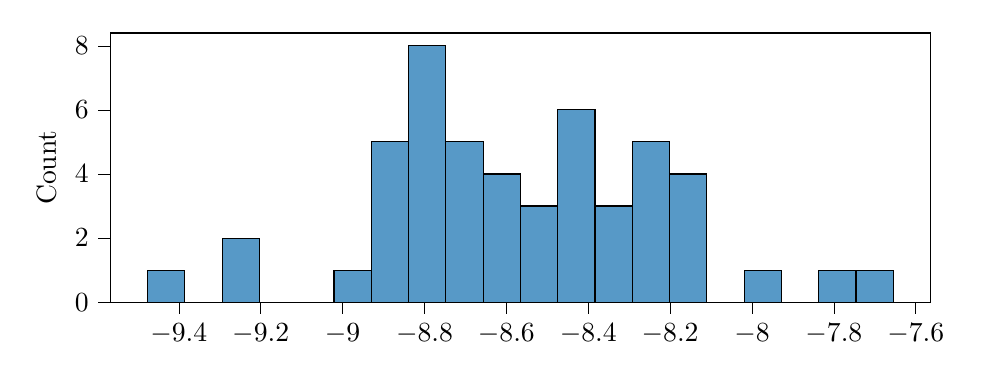
\begin{tikzpicture}
    \definecolor{color0}{rgb}{0.12156862745098,0.466666666666667,0.705882352941177}
    \begin{axis}[
    tick align=outside,
    tick pos=left,
    x grid style={white!69.0196078431373!black},
    xmin=-9.56749670360284, xmax=-7.56375481022318,
    xtick style={color=black},
    y grid style={white!69.0196078431373!black},
    ylabel={Count},
    ymin=0, ymax=8.4,
    ytick style={color=black},
    width=12cm, height=5cm
    ]
    \draw[draw=black,fill=color0,fill opacity=0.75] (axis cs:-9.47641752663104,0) rectangle (axis cs:-9.38533834965923,1);
    \draw[draw=black,fill=color0,fill opacity=0.75] (axis cs:-9.38533834965923,0) rectangle (axis cs:-9.29425917268743,0);
    \draw[draw=black,fill=color0,fill opacity=0.75] (axis cs:-9.29425917268743,0) rectangle (axis cs:-9.20317999571563,2);
    \draw[draw=black,fill=color0,fill opacity=0.75] (axis cs:-9.20317999571563,0) rectangle (axis cs:-9.11210081874383,0);
    \draw[draw=black,fill=color0,fill opacity=0.75] (axis cs:-9.11210081874383,0) rectangle (axis cs:-9.02102164177203,0);
    \draw[draw=black,fill=color0,fill opacity=0.75] (axis cs:-9.02102164177203,0) rectangle (axis cs:-8.92994246480022,1);
    \draw[draw=black,fill=color0,fill opacity=0.75] (axis cs:-8.92994246480022,0) rectangle (axis cs:-8.83886328782842,5);
    \draw[draw=black,fill=color0,fill opacity=0.75] (axis cs:-8.83886328782842,0) rectangle (axis cs:-8.74778411085662,8);
    \draw[draw=black,fill=color0,fill opacity=0.75] (axis cs:-8.74778411085662,0) rectangle (axis cs:-8.65670493388481,5);
    \draw[draw=black,fill=color0,fill opacity=0.75] (axis cs:-8.65670493388481,0) rectangle (axis cs:-8.56562575691301,4);
    \draw[draw=black,fill=color0,fill opacity=0.75] (axis cs:-8.56562575691301,0) rectangle (axis cs:-8.47454657994121,3);
    \draw[draw=black,fill=color0,fill opacity=0.75] (axis cs:-8.47454657994121,0) rectangle (axis cs:-8.38346740296941,6);
    \draw[draw=black,fill=color0,fill opacity=0.75] (axis cs:-8.38346740296941,0) rectangle (axis cs:-8.2923882259976,3);
    \draw[draw=black,fill=color0,fill opacity=0.75] (axis cs:-8.2923882259976,0) rectangle (axis cs:-8.2013090490258,5);
    \draw[draw=black,fill=color0,fill opacity=0.75] (axis cs:-8.2013090490258,0) rectangle (axis cs:-8.110229872054,4);
    \draw[draw=black,fill=color0,fill opacity=0.75] (axis cs:-8.110229872054,0) rectangle (axis cs:-8.0191506950822,0);
    \draw[draw=black,fill=color0,fill opacity=0.75] (axis cs:-8.0191506950822,0) rectangle (axis cs:-7.92807151811039,1);
    \draw[draw=black,fill=color0,fill opacity=0.75] (axis cs:-7.92807151811039,0) rectangle (axis cs:-7.83699234113859,0);
    \draw[draw=black,fill=color0,fill opacity=0.75] (axis cs:-7.83699234113859,0) rectangle (axis cs:-7.74591316416679,1);
    \draw[draw=black,fill=color0,fill opacity=0.75] (axis cs:-7.74591316416679,0) rectangle (axis cs:-7.65483398719499,1);
    \end{axis}
  \end{tikzpicture}
  \caption{Dimension $d=100$}
\end{subfigure}
\begin{subfigure}{\textwidth}
  \centering
  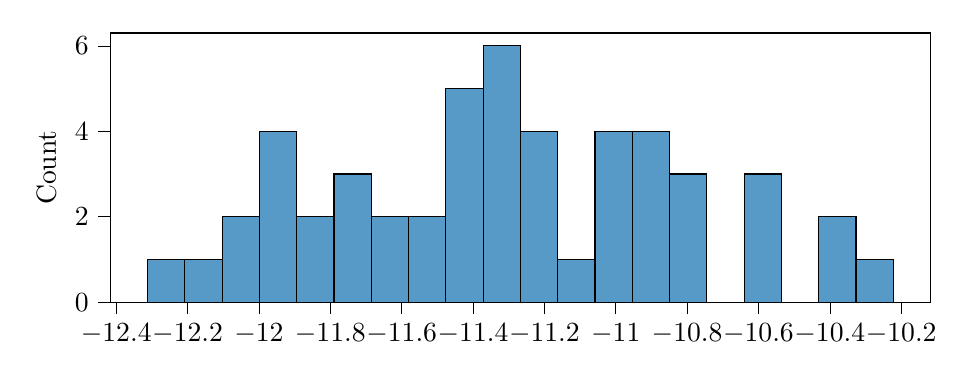
\begin{tikzpicture}
    \definecolor{color0}{rgb}{0.12156862745098,0.466666666666667,0.705882352941177}
    \begin{axis}[
    tick align=outside,
    tick pos=left,
    x grid style={white!69.0196078431373!black},
    xmin=-12.4168122668345, xmax=-10.11762550417,
    xtick style={color=black},
    y grid style={white!69.0196078431373!black},
    ylabel={Count},
    ymin=0, ymax=6.3,
    ytick style={color=black},
    width=12cm, height=5cm
    ]
    \draw[draw=black,fill=color0,fill opacity=0.75] (axis cs:-12.3123037776225,0) rectangle (axis cs:-12.2077952884105,1);
    \draw[draw=black,fill=color0,fill opacity=0.75] (axis cs:-12.2077952884105,0) rectangle (axis cs:-12.1032867991984,1);
    \draw[draw=black,fill=color0,fill opacity=0.75] (axis cs:-12.1032867991984,0) rectangle (axis cs:-11.9987783099864,2);
    \draw[draw=black,fill=color0,fill opacity=0.75] (axis cs:-11.9987783099864,0) rectangle (axis cs:-11.8942698207744,4);
    \draw[draw=black,fill=color0,fill opacity=0.75] (axis cs:-11.8942698207744,0) rectangle (axis cs:-11.7897613315624,2);
    \draw[draw=black,fill=color0,fill opacity=0.75] (axis cs:-11.7897613315624,0) rectangle (axis cs:-11.6852528423503,3);
    \draw[draw=black,fill=color0,fill opacity=0.75] (axis cs:-11.6852528423503,0) rectangle (axis cs:-11.5807443531383,2);
    \draw[draw=black,fill=color0,fill opacity=0.75] (axis cs:-11.5807443531383,0) rectangle (axis cs:-11.4762358639263,2);
    \draw[draw=black,fill=color0,fill opacity=0.75] (axis cs:-11.4762358639263,0) rectangle (axis cs:-11.3717273747143,5);
    \draw[draw=black,fill=color0,fill opacity=0.75] (axis cs:-11.3717273747143,0) rectangle (axis cs:-11.2672188855022,6);
    \draw[draw=black,fill=color0,fill opacity=0.75] (axis cs:-11.2672188855022,0) rectangle (axis cs:-11.1627103962902,4);
    \draw[draw=black,fill=color0,fill opacity=0.75] (axis cs:-11.1627103962902,0) rectangle (axis cs:-11.0582019070782,1);
    \draw[draw=black,fill=color0,fill opacity=0.75] (axis cs:-11.0582019070782,0) rectangle (axis cs:-10.9536934178662,4);
    \draw[draw=black,fill=color0,fill opacity=0.75] (axis cs:-10.9536934178662,0) rectangle (axis cs:-10.8491849286541,4);
    \draw[draw=black,fill=color0,fill opacity=0.75] (axis cs:-10.8491849286541,0) rectangle (axis cs:-10.7446764394421,3);
    \draw[draw=black,fill=color0,fill opacity=0.75] (axis cs:-10.7446764394421,0) rectangle (axis cs:-10.6401679502301,0);
    \draw[draw=black,fill=color0,fill opacity=0.75] (axis cs:-10.6401679502301,0) rectangle (axis cs:-10.5356594610181,3);
    \draw[draw=black,fill=color0,fill opacity=0.75] (axis cs:-10.5356594610181,0) rectangle (axis cs:-10.431150971806,0);
    \draw[draw=black,fill=color0,fill opacity=0.75] (axis cs:-10.431150971806,0) rectangle (axis cs:-10.326642482594,2);
    \draw[draw=black,fill=color0,fill opacity=0.75] (axis cs:-10.326642482594,0) rectangle (axis cs:-10.222133993382,1);
    \end{axis}
  \end{tikzpicture}
  \caption{Dimension $d=200$}
\end{subfigure}
